\documentclass[12pt]{article}
\usepackage{graphicx}
\usepackage{fullpage}
\title{Proposal}
\author{Amy Henry}
\date{January 24, 2013}
\begin{document}
	\maketitle
	\begin{abstract}

	\end{abstract}
	
	\section{Introduction}
	
\par 
Diseases affecting marine species appear to be on the rise, in part due to human activities. Pollution, warming, acidification, and overfishing directly impact many species, but may also increase the incidence and severity of epidemics in corals, urchins, molluscs, marine mammals, and seagrasses \cite{Lafferty:2004hw}(Lafferty et al. 2004).  Marine diseases may thus be another bellwether for anthropogenic influences on ecosystems. 
\par
Marine diseases can also mediate shifts between alternative ecological states. For example, an outbreak of disease in an urchin (Strongylocentrotus purpuratus) barren facilitated the return of a kelp forest off the coast of California by removing the dominant herbivore \cite{Behrens:2004tf}. Conversely, community shifts can alter likelihood of disease, as demonstrated when the removal of predators resulted in abnormally high densities of urchins, where close contact and resource limitation increased susceptibility to an epidemic\cite{Lafferty:2000ti,Lafferty:2004vb} (Lafferty and Kushner 2000, Lafferty 2004). Diseased hosts may have reduced competitive ability, creating opportunities for their competitors to establish and dominate the ecosystem. When the disease host and their competitors are antagonistic ecosystem engineers, like bioturbating species and sediment-stabilizing species, this can completely restructure communities. 
\par
Ecosystem engineers are a subset of keystone species that exert a disproportionate impact on their ecosystem by physically or chemically altering their habitat. These changes to an alternative state can influence greater coastal biogeochemical processes, such as nutrient cycling, productivity, and changes in sediment stability. For example, seagrasses are ecosystem engineers because they alter flow, water quality, and sedimentation conditions, while bioturbators like sand dollars engineer the opposite and increase erosion \cite{DeWitt:2009up}. The goal of my research is to determine how direct and indirect interactions can magnify or modulate the effect of disease and outbreaks on populations and biogeochemical conditions within a system of two competing ecosystem engineer species: eelgrass and sand dollars. 
	
	\section{Background Information}
\par	
	Zostera marina (eelgrass) and other seagrass species are both critical to ecosystem processes and threatened. Z. marina is a temperate shallow water marine species common in the Northeast Pacific and distributed throughout the Northern Hemisphere.  These plants stabilize soft sediment bottoms, create sheltered, complex habitat for both infaunal and pelagic species, and are highly productive. In the 1930s, and again in recent decades, Atlantic populations of Z. marina were decimated by epidemics of eelgrass wasting disease caused by the marine protist Labyrinthula zosterae \cite{Short:1988gx} (Short et al. 1988). Although no widespread loss was observed in the Northeast Pacific in the 1930s, in 2003 the loss of Z. marina within small embayments in the San Juan Archipelago region of the Salish Sea, potentially linked to a disease event, was detected and some of these sites have not fully recovered (Wyllie-Echeverria, et al. in prep, Wyllie-Echeverria et al. 2010).
\par
One species that may respond to Z. marina decline is Dendraster excentricus, the Pacific sand dollar). D. excentricus is a burrowing suspension-feeder that forms dense aggregations that turn over sediment rapidly, rendering habitat hostile to colonizing Z. marina in field experiments \cite{Timko:1976vb}(Backman 1984). Z. marina roots exclude D. excentricus and other hard-bodied burrowing species by reducing their mobility through the sediment \cite{Brenchley:1982wx}. However, bioturbators like D. excentricus can also directly impact plants by uprooting rhizomes and burying new shoots and seedlings. They also may affect the distribution of seagrass indirectly by colonizing space and engineering sediment conditions or flow regimes that exclude Z. marina \cite{DeWitt:2009up}. Z. marina increases the organic content of sediment both by facilitating the settlement of particulate organic matter (POM) from the water column and by leaching dissolved organic matter (DOM) through excretion and decomposition of tissues (Larkum et al 2006). Z. marina bed sediments have more structured oxygenation profiles (Greve et al. 2003) than bare more homogeneously oxygenated bioturbated sediments, which can also affect nutrient transformations. Further, healthy and diseased populations of each species may differ in the profile they generate.
	\begin{figure}
	\begin{center}
	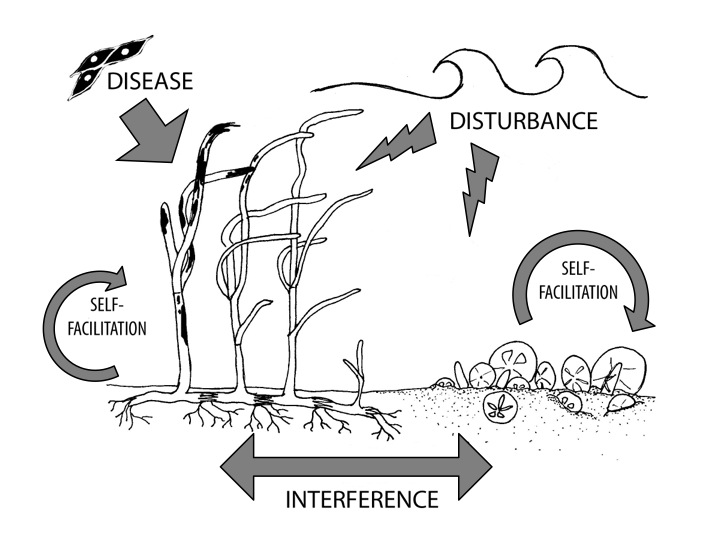
\includegraphics[width=120mm]{Slide1.jpg}
	\caption{\small \sl Hypothesized interactions between sand dollars and eelgrass.}
	\end{center}
	\end{figure}
	
\par
Colonization by bioturbators following a disturbance can slow or stop plant growth, transitioning the habitat to an alternative state \cite{Eklof:2011il}.  In the Netherlands, bioturbating lugworms may colonize and convert Zostera noltii beds to a muddy hollow state where there has been a disturbance of a large enough size, preventing the recolonization of the seagrass (Van der Heide 2012). A similar experiment with D. excentricus and Z. marina (Backman 1984) found that along the boundary between the two species, each excluded the other from areas with established populations, but was able to invade and establish if a disturbance removed and excluded the original species. 
\par
D. excentricus and Z. marina occupy similar depth ranges, flow profiles and sediment types, and both form dense colonies that effectively exclude the opposing species. Z. marina reproduces clonally through rhizome shoots, and thus grows in high density that reduces wave forces on individual plants, reduces erosion and maintains soil conditions. Z. marina has an associated community of many other species of fish, herbivores, epiphytes, and infaunal species. D. excentricus also prefers to live in dense monocultures and facilitates high densities by inducing larval settlement near adults \cite{Highsmith:1982vl}. A statistical analysis of Puget Sound D. excentricus bed fauna did not support a �sand dollar bed community� per se, but did find that some bivalves, polychaetes, and crustaceans are found in higher abundance within sand dollar beds than in bare sand \cite{Smith:1980wz}. Thus, Z. marina beds and D. excentricus beds are alternative states of the same ecosystem. I will examine how these two states affect local community composition.
\par
Zostera japonica was introduced to the Washington coast in the mid 1970s and has spread to shallow bays from Oregon to British Columbia \cite{Posey:1988vh}. Z. japonica has primarily spread through mid-intertidal zones where Z. marina, a lower-intertidal/sub-littoral species, had not previously occupied (Williams 2007). Where their ranges overlap, there is evidence of competition between Z. marina and Z. japonica \cite{Nomme:1991kk}. Though \textit{Z. japonica} is susceptible to infection by \textit{Labyrinthula zosterae}, it has not exhibited the same widespread die-offs observed in \textit{Z. marina} (Short et al. 1993, Garcias-Bonet et al. 2011). Therefore, \textit{Z. japonica} is another candidate to colonize after a potential \textit{Z. marina} epidemic event, and one that could potentially maintain the biodiversity and biogeochemical functioning of seagrass beds, though the species identity differs. 
\par
To understand the nature of the interaction between \textit{Z. marina} and \textit{D. excentricus}, I will examine both direct and indirect competitive effects and how they influence the communities associated with those two species. I will also examine the effects of biogeochemical changes associated with these two species and the potential impacts of \textit{Z. japonica} on this system. 
	
	\section{Research Plan}
	
	I will experimentally examine the specific dynamics of the interaction between D. excentricus and Z. marina to determine how these species structure substrate space. By combining mathematical models and field experiments, I will demonstrate how disease influences community structure within the shallow water marine environment. I hypothesize that D. excentricus colonization will accelerate the decline of diseased Z. marina populations and that areas of diseased plants will be more likely to be colonized by D. excentricus and converted to an alternative state.  The four specific projects I will pursue follow:
	
	\subsection{Interaction between \textit{Zostera marina} and \textit{Dendraster excentricus}}
	
	Through field manipulations, I will determine specific interactions between these competitor species in the absence of disease in the San Juan Archipelago, WA. My objective is to determine (a) if one species is competitively dominant and (b) what processes may influence this interaction. First, I will monitor transects along boundaries between Z. marina and D. excentricus beds to observe possible changes in space occupation through time. I will census communities associated with both of these dominant species through intertidal and diving surveys. Second, I will manipulate 1-m2 quadrats within extant patches of Z. marina and colonies of D. excentricus and monitor the response to disturbance over the course of a growing season (April to September 2013). My manipulations will consist of removal of the existing species and addition of the competitor species (Table 1). I will record population density patterns in both species and associated community fauna. Relative water flow and substrate biogeochemical changes including as nutrient concentrations, particle size, and oxygenation of sediment will be recorded before and after treatments to examine ecosystem-engineering effects and biogeochemical differences. I hypothesize that quadrats will be more likely to shift to an alternative state with disturbance or following the addition of a competitor.
	
	\subsection{Disease effects}
	
	Several sites in the San Juan Archipelago currently differ in their prevalence of eelgrass wasting disease. Because of this variation, I can test disease effects by replicating transect monitoring and experimental manipulations (Table 1) in at least three locations. Comparing these results with those from disease-free transects will allow me to determine how disease mediates this interaction. Comparing abiotic conditions and population characteristics of infected and uninfected sites will provide insight into potential external drivers that bring about lethal disease symptoms in the San Juan Archipelago. To establish causal effects of the disease without introducing the pathogen to new areas, I will selectively replicate experiments in the closed system mesocosms in collaboration with colleagues at Hatfield Marine Science Center in Newport, OR. I hypothesize that wasting disease will weaken competitive performance of Z. marina in the face of interference by D. excentricus. 
	
	\subsection{Spatial models}
	
	I will use models to scale up the findings of experiments and make predictions about eelgrass abundance. I will use my data to parameterize spatial (cellular automata) and non-spatial (Markov) models of probabilistic transitions from one census period to the next among ecological states, for example, occupied by Z. marina or D. excentricus. These models have been shown to accurately predict spatial patterning and community response to local extinction of species among sessile species of the marine rocky intertidal (Wootton 2001 Nature, Wootton 2001 Ecology) With the help of my advisor, Dr. Tim Wootton at the University of Chicago, I will apply these models to predict long-term trends in distribution of eelgrass and sand dollars and the role of spatial structure in their outcome. 
	
	\subsection{Invasive \textit{Zostera japonica}}
	
	I will replicate the experimental setup from Table 1 with Z. japonica in place of D. excentricus to examine how disease alters the competitive dynamic between the two species. I will use sites of co-occurring Z. marina and Z. japonica, or will utilize the mesocosms at Hatfield Marine Science Center to examine competition between Z. marina and Z. japonica with and without disease. I will then use these data to parameterize an invasibility analysis model to predict whether Z. marina will remain in the system or be replaced. 
	
	\subsection{Echinoid and Producer systems}
	
	Bahamas? Cross-system comparisons? 
	
	\subsection{Disease characteristics in \textit{Dendraster excentricus}}
	
	Z. marina wasting disease is not the only disease occurring within this system. In August 2012, I observed apparent declines in the health and population sizes of D. excentricus. The majority of D. excentricus sampled at East Sound, Orcas Island, WA, exhibited epithelial bleaching. Dissections of bleached specimens showed cloudy coelomic fluid, brittle and porous test, and the presence of numerous Vibrio spp. colonies in culture, while healthy specimens had clear coelomic fluid and no Vibrio spp. I will perform inoculations in healthy D. excentricus using isolated cultures from symptomatic D. excentricus to establish pathology, and gather data on transmission rates and field prevalence. My objective is to characterize the key properties of this disease that could alter the interaction between Z. marina and D. excentricus in the presence of either or both diseases. I will determine the environmental factors that precipitate both diseases and examine whether they covary or may alternate in a boom-bust fashion. This addition of a second disease to my system will add complexity to my models. 
	
	\section{Summary}
	
	Writing a summary is fun!
	
	\bibliographystyle{plain}
	\bibliography{FullLibBib}
	
	
	
\end{document}